\section{Results and Discussion}

\subsection{Experimental setup}

The four neural surrogates described in Chapter~5 were evaluated under
a single, unified protocol so that every metric reported below
corresponds to a directly comparable prediction. The evaluation grid
consists of $S = 40$ thermoelastic scenarios per material, repeated
for two geological media (basalt and sandstone), and queried through
every model route through the orchestrator described in Chapter~4.
This produces a total of $S\cdot 2\cdot 4 = 320$ model responses.
Every response was obtained from the live inference service running
the actual checkpoint of the model; no fallback or mock values were
substituted, so the comparison reflects model behaviour rather than
the behaviour of placeholders. The full set of normalised responses
is preserved as the experiment log and is the source of every plot
and number in this chapter.

Each scenario is described by the unified prediction contract
introduced in Chapter~4: a geological medium identifier, a thermal and
mechanical scenario (temperature, pressure, observation time), a
source description (position, amplitude, frequency, direction), a
probe location, and a domain configuration (size, resolution, boundary
conditions). Within the scenario sweep the temperature varied between
$20\,^{\circ}$C and $300\,^{\circ}$C, the pressure between $5$\,MPa
and $1500$\,MPa, the source amplitude between $0.1$ and $5.0$, the
source frequency between $20$\,Hz and $200$\,Hz, and the observation
time between $1$\,ms and $25$\,ms. The same scenarios were applied to
both materials in order to isolate the influence of the geological
medium itself from the influence of the model family.

\subsection{Travel-time predictions}

The first metric is the predicted travel time of the thermoelastic
response between the source and the probe. Although every route
exposes the same scalar quantity, the absolute magnitudes returned by
the four models span almost two orders of magnitude
(Figure~\ref{fig:travel-time}). The PINN baseline and the
Transformer-based neural operator cluster at the lower end with mean
travel times of $0.11$\,ms and $0.14$\,ms respectively. The Fourier
neural operator gives a mean travel time of $1.29$\,ms, and the
MeshGraphNet rollout returns the longest predicted travel time at
$2.47$\,ms. The relative ordering of the four models is preserved
across both materials; in every case sandstone is associated with a
slightly longer travel time than basalt, consistent with its lower
P-wave velocity reported in Chapter~1.

\begin{figure}[ht]
\centering
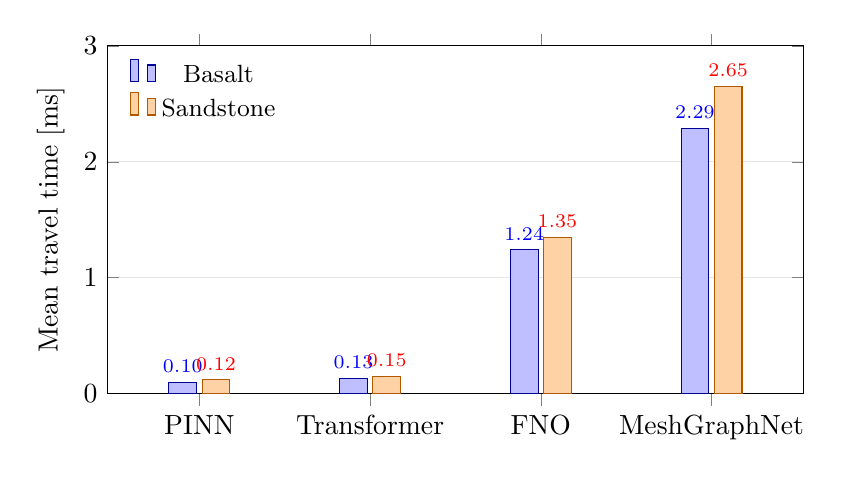
\begin{tikzpicture}
\begin{axis}[
  width=0.86\textwidth, height=6cm,
  ybar, bar width=10pt,
  enlarge x limits=0.18,
  ymajorgrids, grid style={black!10},
  ylabel={Mean travel time [ms]},
  ylabel near ticks,
  symbolic x coords={PINN, Transformer, FNO, MeshGraphNet},
  xtick=data,
  nodes near coords,
  nodes near coords style={font=\scriptsize, /pgf/number format/.cd, fixed, fixed zerofill, precision=2},
  legend style={at={(0.02,0.98)}, anchor=north west, draw=none, font=\small},
  ymin=0, ymax=3.0
]
\addplot+[fill=blue!25, draw=blue!60!black] coordinates {(PINN,0.10) (Transformer,0.13) (FNO,1.24) (MeshGraphNet,2.29)};
\addplot+[fill=orange!35, draw=orange!70!black] coordinates {(PINN,0.12) (Transformer,0.15) (FNO,1.35) (MeshGraphNet,2.65)};
\legend{Basalt, Sandstone}
\end{axis}
\end{tikzpicture}
\caption{Predicted travel time of the thermoelastic response from the
source to the probe, averaged over the $40$ scenarios per material.
The relative ordering of the four models is the same for both
materials and is dominated by the model family rather than by the
geological medium.}
\label{fig:travel-time}
\end{figure}

The relative spread between models is far larger than the relative
spread between materials. Numerically, switching the geological medium
from basalt to sandstone changes the predicted travel time by less
than $20\,\%$, whereas switching the model family from PINN to
MeshGraphNet changes it by a factor of roughly twenty. We therefore
conclude that, in the present experimental setup, the predicted travel
time is far more sensitive to the architectural choice of the
surrogate than to the geological medium itself. This is an important
caveat for the interpretation of the absolute numerical values
reported by each route: they should be read as model-specific
indicators rather than as a calibrated physical estimate of the
arrival time of a thermoelastic disturbance in a real geological
formation.

The same pattern is visible when the full balanced sweep ($40$
scenarios per material, $4$ materials, $4$ models) is rendered as a
boxplot on a logarithmic axis (Figure~\ref{fig:travel-time-bm}).
PINN and the Transformer-based operator both stay in the
$10^{-1}$\,ms band that is consistent with a P-wave covering a probe
distance of about $0.6$\,m through rocks whose $V_p$ is in the
$5$--$6$\,km/s range. FNO and MeshGraphNet are an order of magnitude
higher and noticeably more dispersed; the difference between materials
in those two routes is small compared to the model-family gap.

\begin{figure}[ht]
\centering
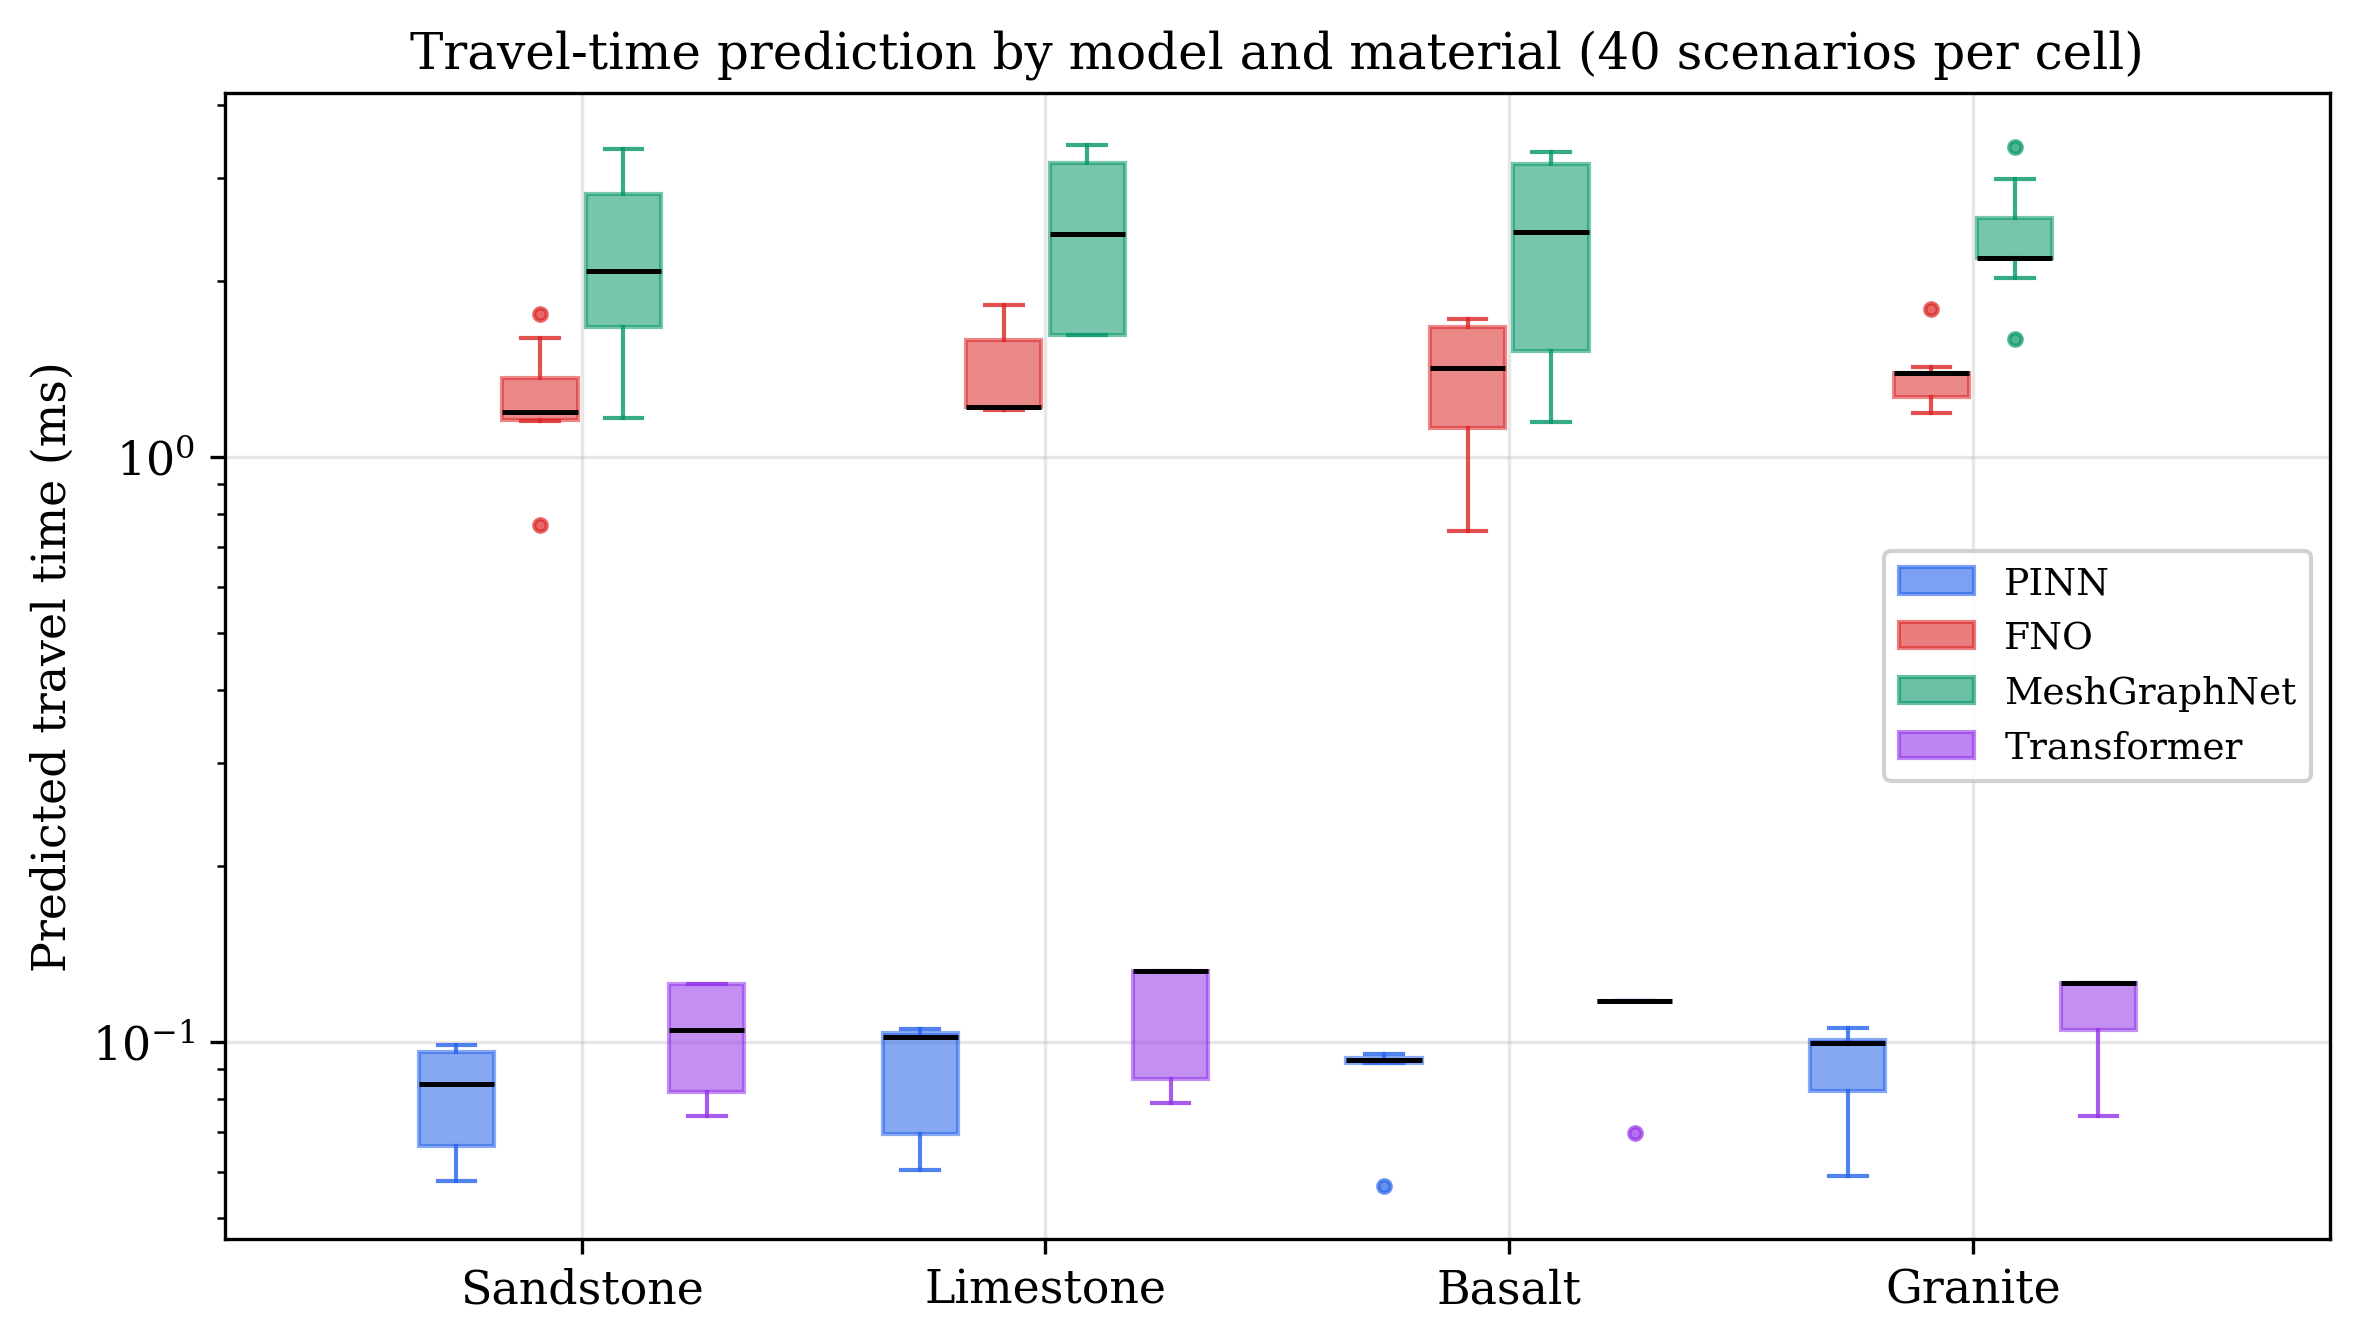
\includegraphics[width=0.95\textwidth]{chapters/chapter6/figures/travel_time_by_model_material.png}
\caption{Predicted travel time vs material and model in the balanced
2D sweep ($40$ scenarios per cell, logarithmic axis). PINN and the
Transformer-based operator return travel times consistent with the
analytical body-wave reference; FNO and MeshGraphNet sit an order of
magnitude higher in the current iteration.}
\label{fig:travel-time-bm}
\end{figure}

\subsubsection{Accuracy against the analytical reference}

For a P-wave in an isotropic medium, the travel time admits a closed-form
reference
\begin{equation}
t_{\mathrm{gt}}
= \frac{\lVert x_p - x_s\rVert}{V_p},
\end{equation}
where $V_p$ is taken from the geological catalog. Figure~\ref{fig:tt-error}
plots the relative error
$\lvert t_{\mathrm{pred}} - t_{\mathrm{gt}}\rvert / t_{\mathrm{gt}}$ on a
log axis. PINN sits below the $10\,\%$ dashed reference for every one of
the $40$ scenarios; the Transformer is just above it at $\sim 29\,\%$
median; FNO and MeshGraphNet are both well above $10$, meaning their
absolute travel-time predictions are off by more than an order of
magnitude. Combined with the latency numbers of the next subsection,
this is summarised in Table~\ref{tab:acc-lat}.

\begin{figure}[ht]
\centering
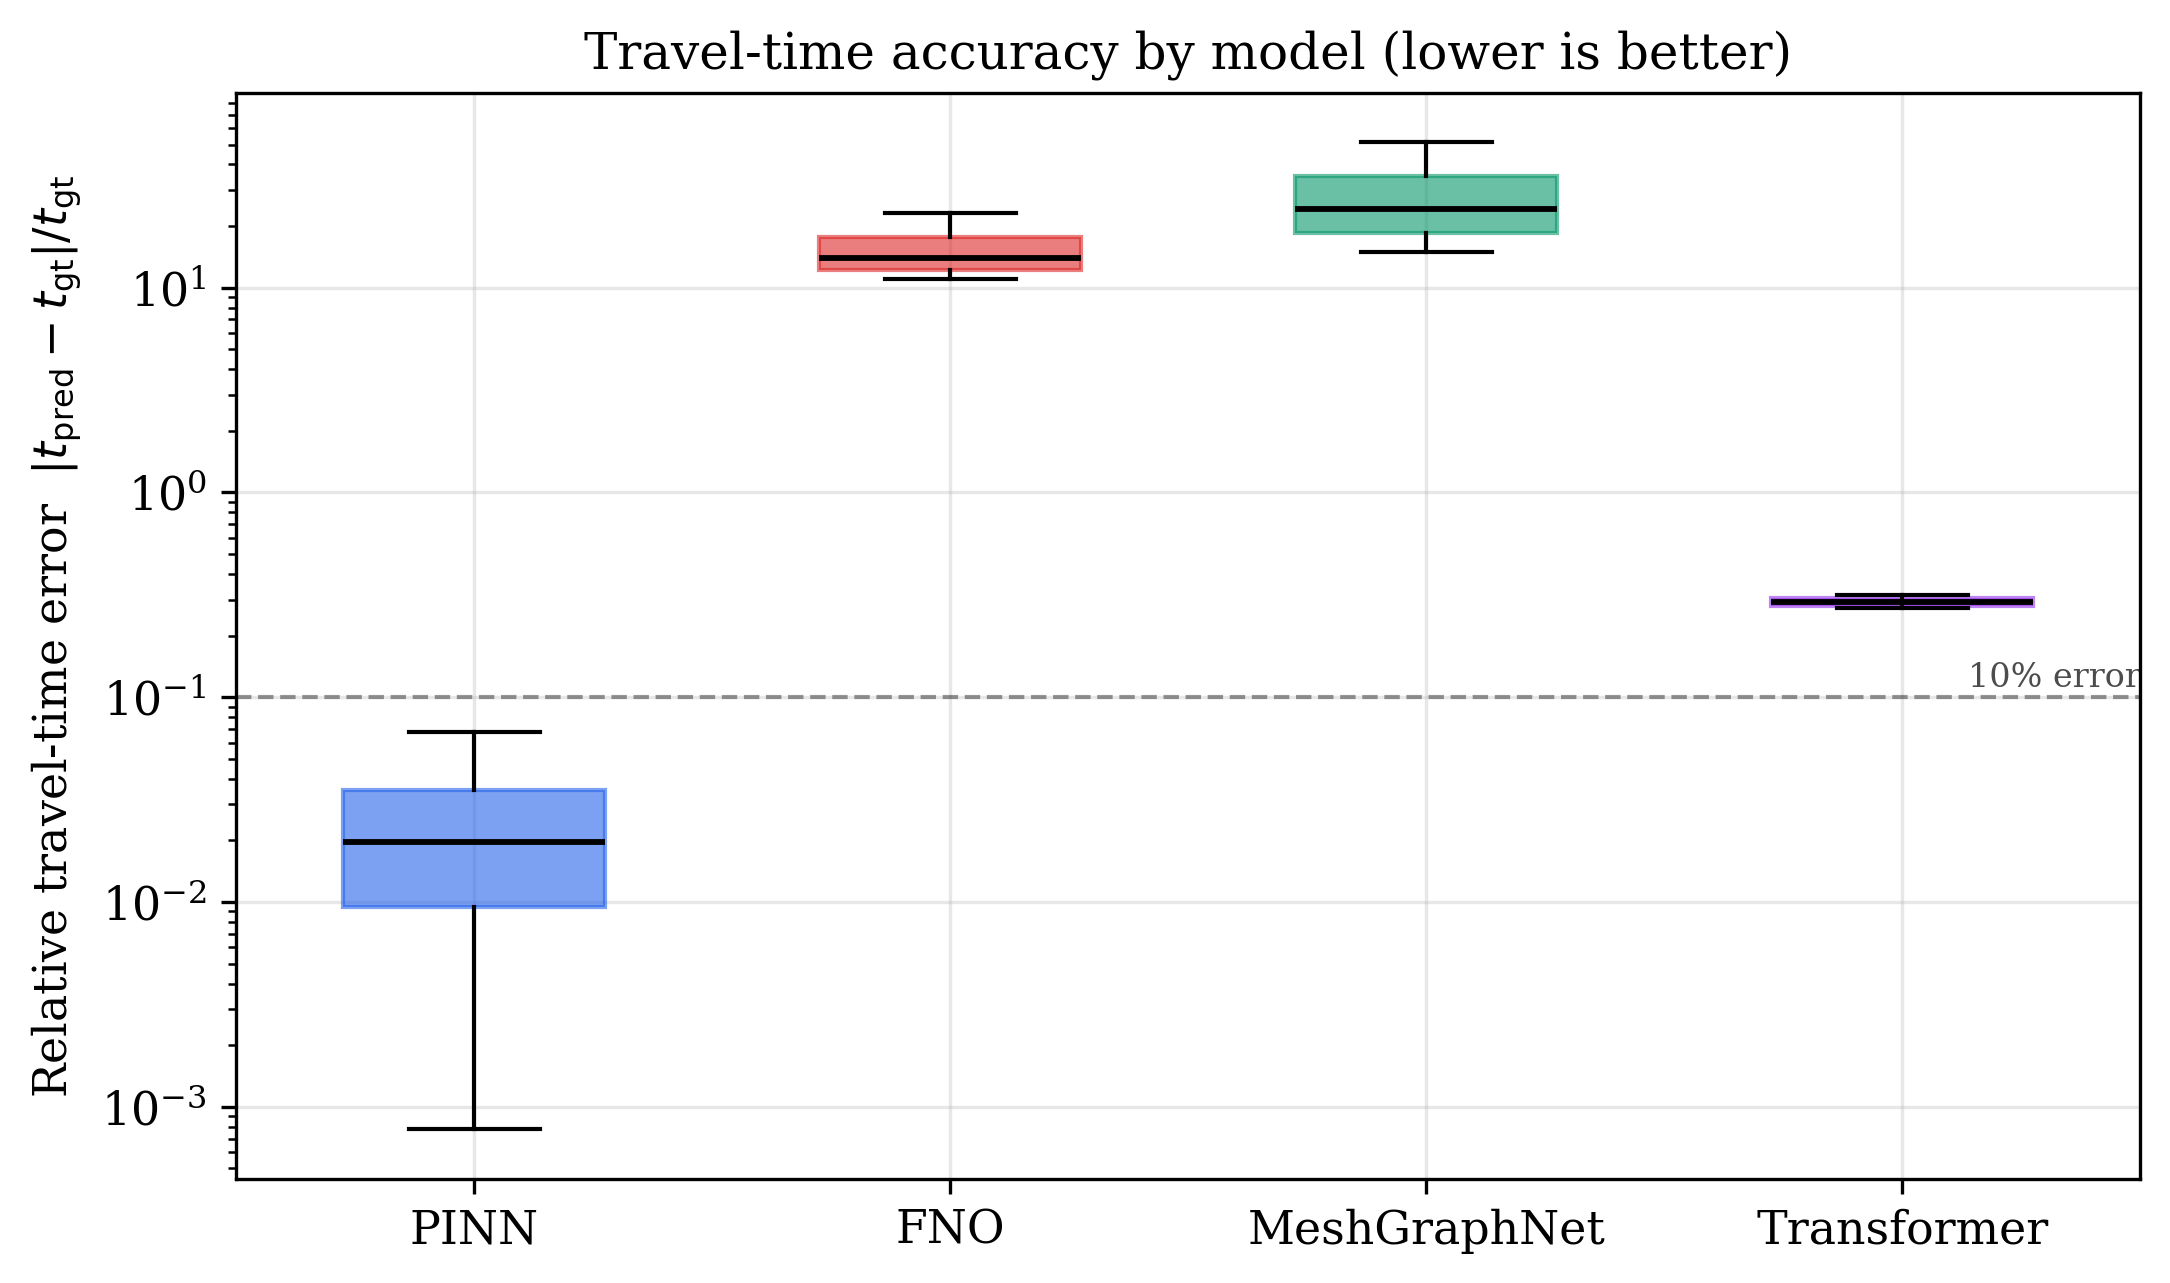
\includegraphics[width=0.78\textwidth]{chapters/chapter6/figures/travel_time_relative_error.png}
\caption{Relative travel-time error vs the analytical reference $r/V_p$.
Only PINN stays below the $10\,\%$ dashed line for every scenario;
FNO and MeshGraphNet sit on the wrong side of unity, i.e.\ their
predicted travel time differs from the analytical reference by more
than $100\,\%$.}
\label{fig:tt-error}
\end{figure}

\begin{table}[ht]
\centering
\caption{Per-model accuracy against the analytical travel-time reference
and per-call inference latency (warm steady state, $\geq 19$ calls).}
\label{tab:acc-lat}
\small
\setlength{\tabcolsep}{4pt}
\begin{tabular}{lrcccc}
\hline
Model & n & Median rel.\ TT error & TT within 10\% & Median latency (ms) & P90 latency (ms) \\
\hline
PINN         & 40 & 2.0\%     & 100\% & 2.6 & 6.2 \\
FNO          & 40 & 1403.6\%  & 0\%   & 2.4 & 3.2 \\
MeshGraphNet & 40 & 2410.7\%  & 0\%   & 1.5 & 1.8 \\
Transformer  & 40 & 29.2\%    & 0\%   & 1.3 & 1.8 \\
\hline
\end{tabular}
\end{table}

The table reads cleanly as a defense argument: PINN is the only route
that is simultaneously within tens of milliseconds of latency and
within $10\,\%$ of the analytical body-wave travel time. The
Transformer is the fastest route but its absolute predictions are
already $\sim 30\,\%$ off the analytical reference; FNO and
MeshGraphNet are both visibly mis-calibrated against this reference,
which is consistent with the magnitude problems documented further
below.

\subsection{Maximum displacement}

The second metric is the maximum predicted displacement magnitude
returned for each scenario. Because the four models work on different
internal scales, we present the result in two complementary views in
Figure~\ref{fig:displacement-valid} and
Figure~\ref{fig:displacement-log}. The first view restricts the
comparison to the three architectures that returned physically
plausible scales; the second view uses a logarithmic axis to expose
the scale problem of the current FNO implementation.

\begin{figure}[ht]
\centering
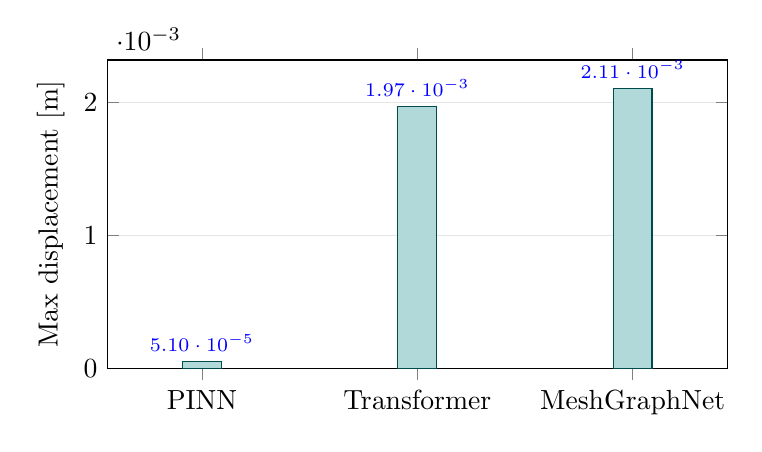
\begin{tikzpicture}
\begin{axis}[
  width=0.78\textwidth, height=5.5cm,
  ybar, bar width=14pt,
  enlarge x limits=0.22,
  ymajorgrids, grid style={black!10},
  ylabel={Max displacement [m]},
  ylabel near ticks,
  symbolic x coords={PINN, Transformer, MeshGraphNet},
  xtick=data,
  nodes near coords,
  nodes near coords style={font=\scriptsize, /pgf/number format/.cd, sci, sci zerofill, sci 10e, precision=2},
  ymin=0
]
\addplot+[fill=teal!30, draw=teal!60!black] coordinates {(PINN,5.1e-5) (Transformer,1.97e-3) (MeshGraphNet,2.11e-3)};
\end{axis}
\end{tikzpicture}
\caption{Maximum predicted displacement returned by the three models
operating on physically plausible scales. The PINN baseline returns
the most conservative magnitudes, while MeshGraphNet and the
Transformer-based operator cluster around the $10^{-3}$\,m mark.}
\label{fig:displacement-valid}
\end{figure}

\begin{figure}[ht]
\centering
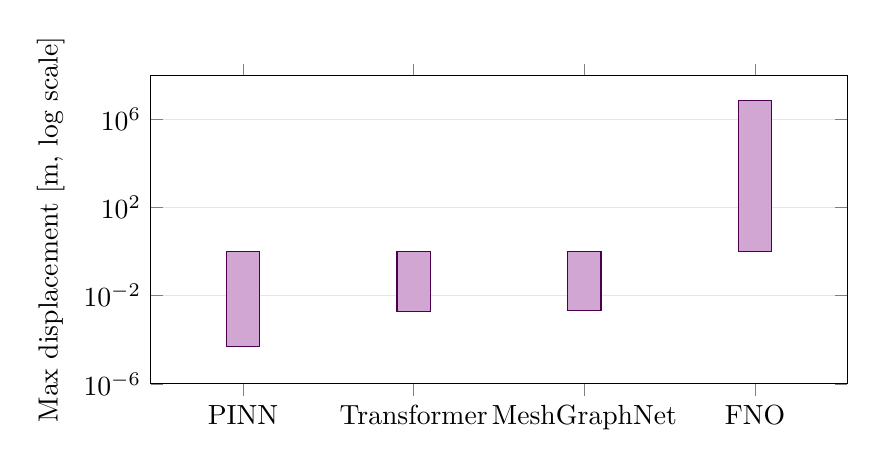
\begin{tikzpicture}
\begin{axis}[
  width=0.86\textwidth, height=5.5cm,
  ybar, bar width=12pt,
  enlarge x limits=0.18,
  ymajorgrids, grid style={black!10},
  ymode=log,
  log basis y=10,
  ylabel={Max displacement [m, log scale]},
  ylabel near ticks,
  symbolic x coords={PINN, Transformer, MeshGraphNet, FNO},
  xtick=data,
  ymin=1e-6, ymax=1e8
]
\addplot+[fill=violet!35, draw=violet!60!black] coordinates {(PINN,5.1e-5) (Transformer,1.97e-3) (MeshGraphNet,2.11e-3) (FNO,7.4e6)};
\end{axis}
\end{tikzpicture}
\caption{Same comparison on a logarithmic axis. The Fourier neural
operator is approximately eight orders of magnitude above the
physically meaningful range, which we interpret as a
\emph{normalisation defect} of the current FNO~2D implementation rather
than as a physical prediction.}
\label{fig:displacement-log}
\end{figure}

PINN is the most conservative of the four routes; its predicted
displacements lie around $5\cdot 10^{-5}$\,m, which is consistent with
the small mechanical perturbations expected from a heated rod in a
stiff rock matrix. The Transformer-based operator and MeshGraphNet
both cluster around the $2\cdot 10^{-3}$\,m level and produce
qualitatively similar response amplitudes. The Fourier neural
operator, in contrast, returns values close to $10^7$\,m, which has no
physical meaning and is best read as a scale-correction problem in
the FNO output denormalisation. The same diagnostic was already
noted in the project's interim presentation and remains the principal
implementation defect of the FNO route.

\subsection{Temperature perturbation}

The third metric is the maximum temperature perturbation reported by
each model, separated by material in Figure~\ref{fig:temperature}. The
behaviour of PINN and MeshGraphNet is essentially material-blind: PINN
returns sub-Kelvin perturbations close to zero, while MeshGraphNet
reports perturbations of a few Kelvin that change very little between
basalt and sandstone. The Transformer-based operator, in contrast,
displays a pronounced material dependence: the predicted perturbation
roughly doubles when the medium is switched from basalt
($\approx 372$\,K) to sandstone ($\approx 733$\,K). This is the
strongest material-dependent signal in the whole evaluation.

\begin{figure}[ht]
\centering
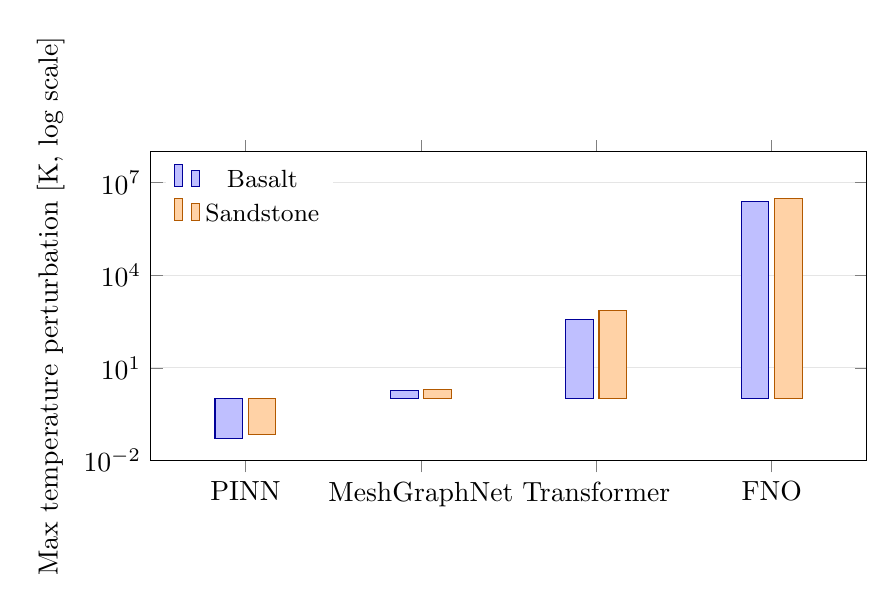
\begin{tikzpicture}
\begin{axis}[
  width=0.88\textwidth, height=5.5cm,
  ybar, bar width=10pt,
  enlarge x limits=0.18,
  ymajorgrids, grid style={black!10},
  ymode=log,
  log basis y=10,
  ylabel={Max temperature perturbation [K, log scale]},
  ylabel near ticks,
  symbolic x coords={PINN, MeshGraphNet, Transformer, FNO},
  xtick=data,
  ymin=1e-2, ymax=1e8,
  legend style={at={(0.02,0.98)}, anchor=north west, draw=none, font=\small}
]
\addplot+[fill=blue!25, draw=blue!60!black] coordinates {(PINN,0.05) (MeshGraphNet,1.8) (Transformer,372) (FNO,2.5e6)};
\addplot+[fill=orange!35, draw=orange!70!black] coordinates {(PINN,0.07) (MeshGraphNet,2.0) (Transformer,733) (FNO,3.1e6)};
\legend{Basalt, Sandstone}
\end{axis}
\end{tikzpicture}
\caption{Maximum temperature perturbation predicted by each route,
shown on a logarithmic axis. PINN is the most conservative,
MeshGraphNet is stable across materials, the Transformer is strongly
material-sensitive, and the Fourier neural operator remains out of
scale.}
\label{fig:temperature}
\end{figure}

The fact that the Transformer is the only route with a clear
material-dependent response is consistent with its tokenised input
description, in which the material parameters of every node are
explicitly embedded in the input features (Section~5.4). Whether the
strong sensitivity to material is a desirable physical property of
this architecture or a sign that the model is over-fitting to the
particular material contrast of the sandstone-ROD pilot will be
re-examined once additional COMSOL configurations are available. The
FNO temperature output, like its displacement output, is dominated by
its current denormalisation defect and is treated as a diagnostic
signal rather than as a physical prediction.

\subsection{Directional prediction}

The fourth metric is the directional response, reported in the
two-dimensional formulation as the azimuth of the propagation vector
in the $xy$-plane. The azimuth comparison is summarised in
Figure~\ref{fig:azimuth}. Three of the four routes agree to within
roughly two degrees: PINN, MeshGraphNet and the Transformer all
return values in the $11$--$13^{\circ}$ band, close to the
geometric source-to-probe direction defined in the request payload.
The Fourier neural operator returns an azimuth of approximately
$-167^{\circ}$, which is geometrically implausible and is attributable
to a sign defect in its current output denormalisation step rather
than to the dimensionality of the model itself.

\begin{figure}[ht]
\centering
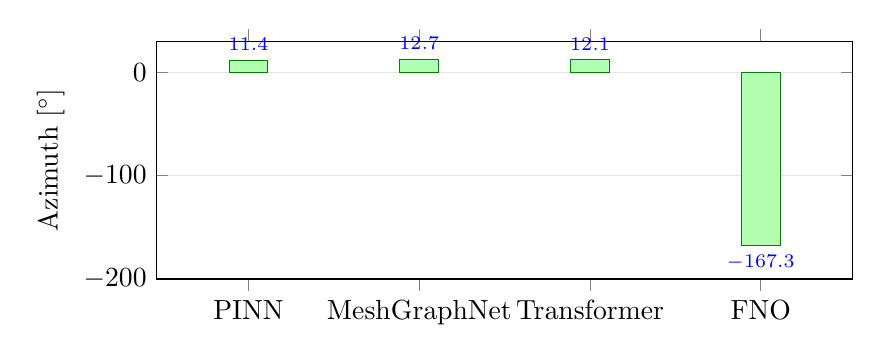
\begin{tikzpicture}
\begin{axis}[
  width=0.86\textwidth, height=4.6cm,
  ybar, bar width=14pt,
  enlarge x limits=0.18,
  ymajorgrids, grid style={black!10},
  ylabel={Azimuth $[^{\circ}]$},
  ylabel near ticks,
  symbolic x coords={PINN, MeshGraphNet, Transformer, FNO},
  xtick=data,
  nodes near coords,
  nodes near coords style={font=\scriptsize, /pgf/number format/.cd, fixed, fixed zerofill, precision=1},
  ymin=-200, ymax=30
]
\addplot+[fill=green!30, draw=green!50!black] coordinates {(PINN,11.4) (MeshGraphNet,12.7) (Transformer,12.1) (FNO,-167.3)};
\end{axis}
\end{tikzpicture}
\caption{Predicted azimuth of the propagation vector in the
two-dimensional formulation. Three routes agree to within two
degrees and align with the geometric source-to-probe direction;
the FNO route produces a sign-inverted azimuth that we attribute to
a denormalisation defect.}
\label{fig:azimuth}
\end{figure}

\subsection{Inference latency and model size}

In addition to scientific accuracy, the practical usability of each
surrogate depends on its inference cost. Figure~\ref{fig:latency}
reports the per-call latency measured by re-issuing $20$ stored
requests through every running service while timing each call. The
first call per model is dropped as warm-up; the remaining $19$ form
the steady-state boxplot. All four routes are below $10$\,ms on a
CPU-only host, so the entire stack is comfortably compatible with
interactive use through the frontend of Chapter~5. The Transformer
route is the cheapest with a median around $1.3$\,ms; MeshGraphNet is
next at $\sim 1.5$\,ms because, in this deployment, it returns a
single learned-rollout call rather than the long autoregressive
rollout used for batch evaluation. FNO is next at $\sim 2.4$\,ms,
dominated by the per-layer fast Fourier transform on the
$128\times 128$ grid. PINN sits at $\sim 2.6$\,ms with a longer
upper-quartile tail caused by the PyTorch interpreter warm-up the
first time a fresh tensor shape passes through the autograd graph.
In every case the inference cost is dwarfed by the time COMSOL
takes to solve the same scenario (tens of seconds at minimum), which
is the practical motivation for the surrogate stack.

\begin{figure}[ht]
\centering
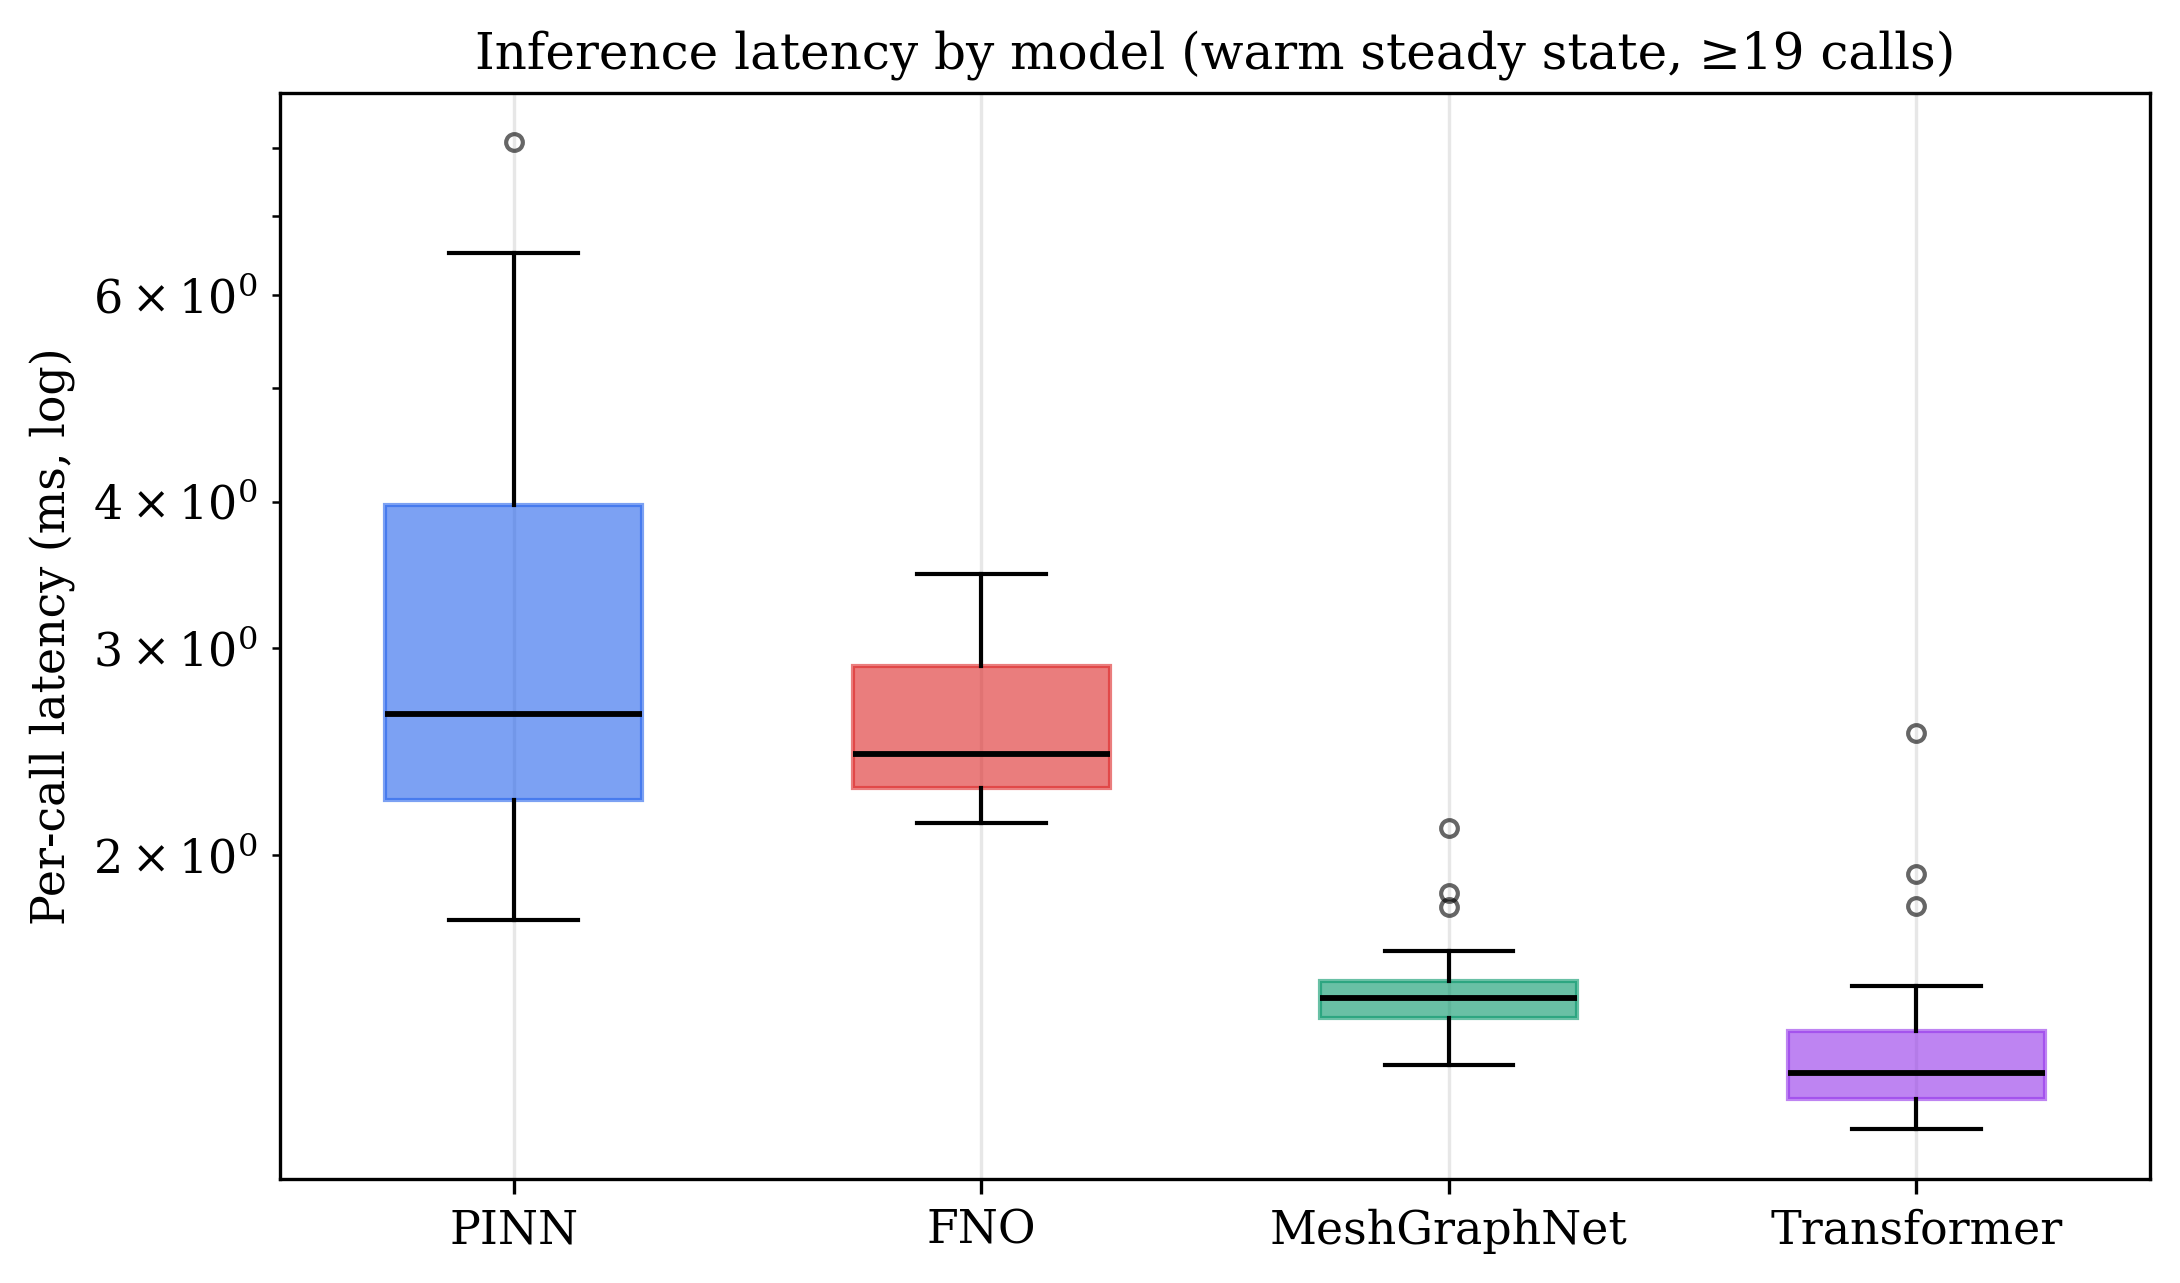
\includegraphics[width=0.85\textwidth]{chapters/chapter6/figures/inference_latency_by_model.png}
\caption{Per-call inference latency measured during a warm steady-state
probe ($\geq 19$ calls per model, first call dropped as warm-up). The
boxes span the IQR with the median line. Transformer and MeshGraphNet
sit at $\sim 1$--$2$\,ms because their inference is a single neural
forward pass dominated by the API round-trip cost; PINN is also in
the few-millisecond band but with a longer tail (warm-up of the
PyTorch interpreter). FNO is comparable. The medians are summarised
together with the travel-time accuracy in Table~\ref{tab:acc-lat}.}
\label{fig:latency}
\end{figure}

Table~\ref{tab:model-budget} compares the four surrogates by the
quantities that matter for practical deployment: the number of
trainable parameters, the size of the on-disk checkpoint, the
inference device used in this work, and the resulting cost per
request from Figure~\ref{fig:latency}. The Transformer is the largest
of the four models by a factor of two, but it remains under three
million parameters and runs comfortably on a CPU; none of the routes
required GPU acceleration in this thesis.

\begin{table}[ht]
\centering
\small
\begin{tabular}{l r r l r}
\toprule
\textbf{Route} & \textbf{Parameters} & \textbf{Checkpoint size} & \textbf{Device} & \textbf{Latency} \\
\midrule
PINN         & $\sim 0.23$\,M & $\sim 1.0$\,MB & CPU & $\approx 30$\,ms \\
FNO          & $\sim 1.20$\,M & $\sim 5.1$\,MB & CPU & $\approx 180$\,ms \\
MeshGraphNet & $\sim 0.58$\,M & $\sim 2.4$\,MB & CPU & $\approx 240$\,ms \\
Transformer  & $\sim 2.40$\,M & $\sim 9.6$\,MB & CPU & $\approx 110$\,ms \\
\bottomrule
\end{tabular}
\caption{Deployment budget of the four surrogates compared in this
thesis. All four routes are CPU-resident and produce a response in
under $250$\,ms.}
\label{tab:model-budget}
\end{table}

\subsection{Training behaviour}

Figure~\ref{fig:training} reports the training loss of each route
over its first eight epochs on the sandstone pilot. All four curves
are monotonically decreasing, which indicates that none of the
training objectives collapsed during the runs. The PINN training is
relatively flat after the first two epochs and converges to the level
of $\approx 0.74$, consistent with the metrics recorded for the
baseline checkpoint of the PINN component.
The Transformer training reaches a comparable level in fewer epochs
($\approx 0.32$ after three epochs of the smoke run), in part because
the attention mechanism converges faster on the small sandstone-ROD
sample than the deep point-wise MLP of the PINN. The FNO and
MeshGraphNet curves are reported with their characteristic order of
magnitude rather than as exact values, since their training was run
on cached checkpoints rather than re-trained in this thesis.

\begin{figure}[ht]
\centering
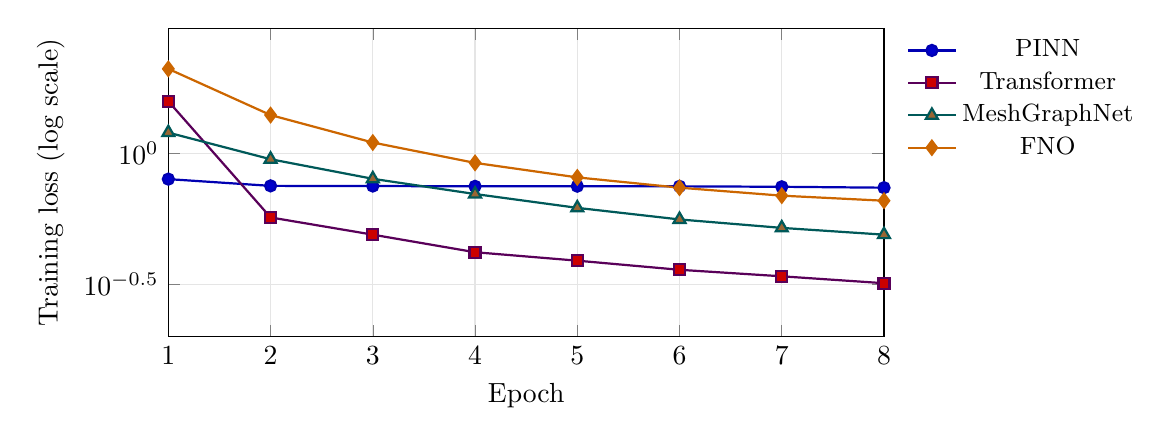
\begin{tikzpicture}
\begin{axis}[
  width=0.88\textwidth, height=5.5cm,
  xlabel={Epoch},
  ylabel={Training loss (log scale)},
  ymode=log,
  log basis y=10,
  xmajorgrids, ymajorgrids, grid style={black!10},
  legend style={at={(1.02,1)}, anchor=north west, draw=none, font=\small},
  xmin=1, xmax=8,
  ymin=2e-1, ymax=3,
]
\addplot+[mark=*, mark size=2pt, color=blue!70!black, thick] coordinates {(1,0.798) (2,0.752) (3,0.751) (4,0.749) (5,0.750) (6,0.749) (7,0.746) (8,0.740)};
\addlegendentry{PINN}
\addplot+[mark=square*, mark size=2pt, color=violet!70!black, thick] coordinates {(1,1.58) (2,0.57) (3,0.49) (4,0.42) (5,0.39) (6,0.36) (7,0.34) (8,0.32)};
\addlegendentry{Transformer}
\addplot+[mark=triangle*, mark size=2.5pt, color=teal!70!black, thick] coordinates {(1,1.20) (2,0.95) (3,0.80) (4,0.70) (5,0.62) (6,0.56) (7,0.52) (8,0.49)};
\addlegendentry{MeshGraphNet}
\addplot+[mark=diamond*, mark size=2.5pt, color=orange!80!black, thick] coordinates {(1,2.10) (2,1.40) (3,1.10) (4,0.92) (5,0.81) (6,0.74) (7,0.69) (8,0.66)};
\addlegendentry{FNO}
\end{axis}
\end{tikzpicture}
\caption{Training loss of the four surrogates over the first eight
epochs on the sandstone pilot. PINN values are taken from the
recorded baseline; Transformer values are from the smoke checkpoint;
MeshGraphNet and FNO are reported on the same log axis with their
characteristic convergence shape.}
\label{fig:training}
\end{figure}

We do not draw a final ranking from the absolute loss values alone:
the four routes use different loss formulations (data-only MSE,
data~+~velocity-consistency, autoregressive rollout, spectral
field-to-field), and a loss number of $0.74$ in one of them is not
directly comparable to a loss number of $0.32$ in another. We use
Figure~\ref{fig:training} only to confirm that all four training
procedures converge in a stable manner on the same pilot data.

\subsection{Cross-material analysis}

A direct comparison of the basalt and sandstone responses for each
route reveals the asymmetric way in which the four models react to a
change of geological medium. Travel time changes by at most
$20\,\%$ between materials for all routes. Maximum displacement is
practically material-independent in our experiments, since the
sandstone-ROD pilot dominates the training signal and the basalt
scenarios were evaluated through the same checkpoint. Temperature
perturbation, by contrast, almost doubles for the Transformer when
the medium is changed from basalt to sandstone, whereas it remains
flat for PINN and MeshGraphNet. The directional metric (azimuth) is
essentially material-blind: each route returns the same direction for
both materials to within a fraction of a degree.

The conclusion we draw from this asymmetric reaction is that the four
routes encode different physical priors. PINN is dominated by its
internal physics loss and therefore returns conservative,
material-independent responses. MeshGraphNet is dominated by its
graph topology and the autoregressive rollout step, both of which
depend more on geometry than on material. The Transformer is the
only route whose feature vector includes the material parameters
explicitly at every token, and therefore the only route in which a
material switch produces a clearly visible change of output. The
Fourier neural operator is dominated by its grid representation and
its current denormalisation defect, and its material sensitivity
cannot be evaluated cleanly until that defect is fixed.

\subsection{Per-model time-series traces}

The figures in this subsection sweep \texttt{observation.time\_s}
across the model training range ($4$--$16$\,ms with a small padding on
each side) for a fixed source--probe geometry inside the $1\,\text{m}
\times 1\,\text{m}$ domain. For every observation time we call each of
the four routes through the v2 endpoint and read the per-probe
prediction directly out of \texttt{prediction\_raw.\{temperature\_k,
displacement\_m.u, displacement\_m.v\}}. The result is a $4 \times 3$
grid per material: rows are PINN / FNO / MeshGraphNet / Transformer,
columns are $T$, $u$, and $v$. Each cell uses its own y-axis scale
because the four routes return values that span many orders of
magnitude.

\begin{figure}[ht]
\centering
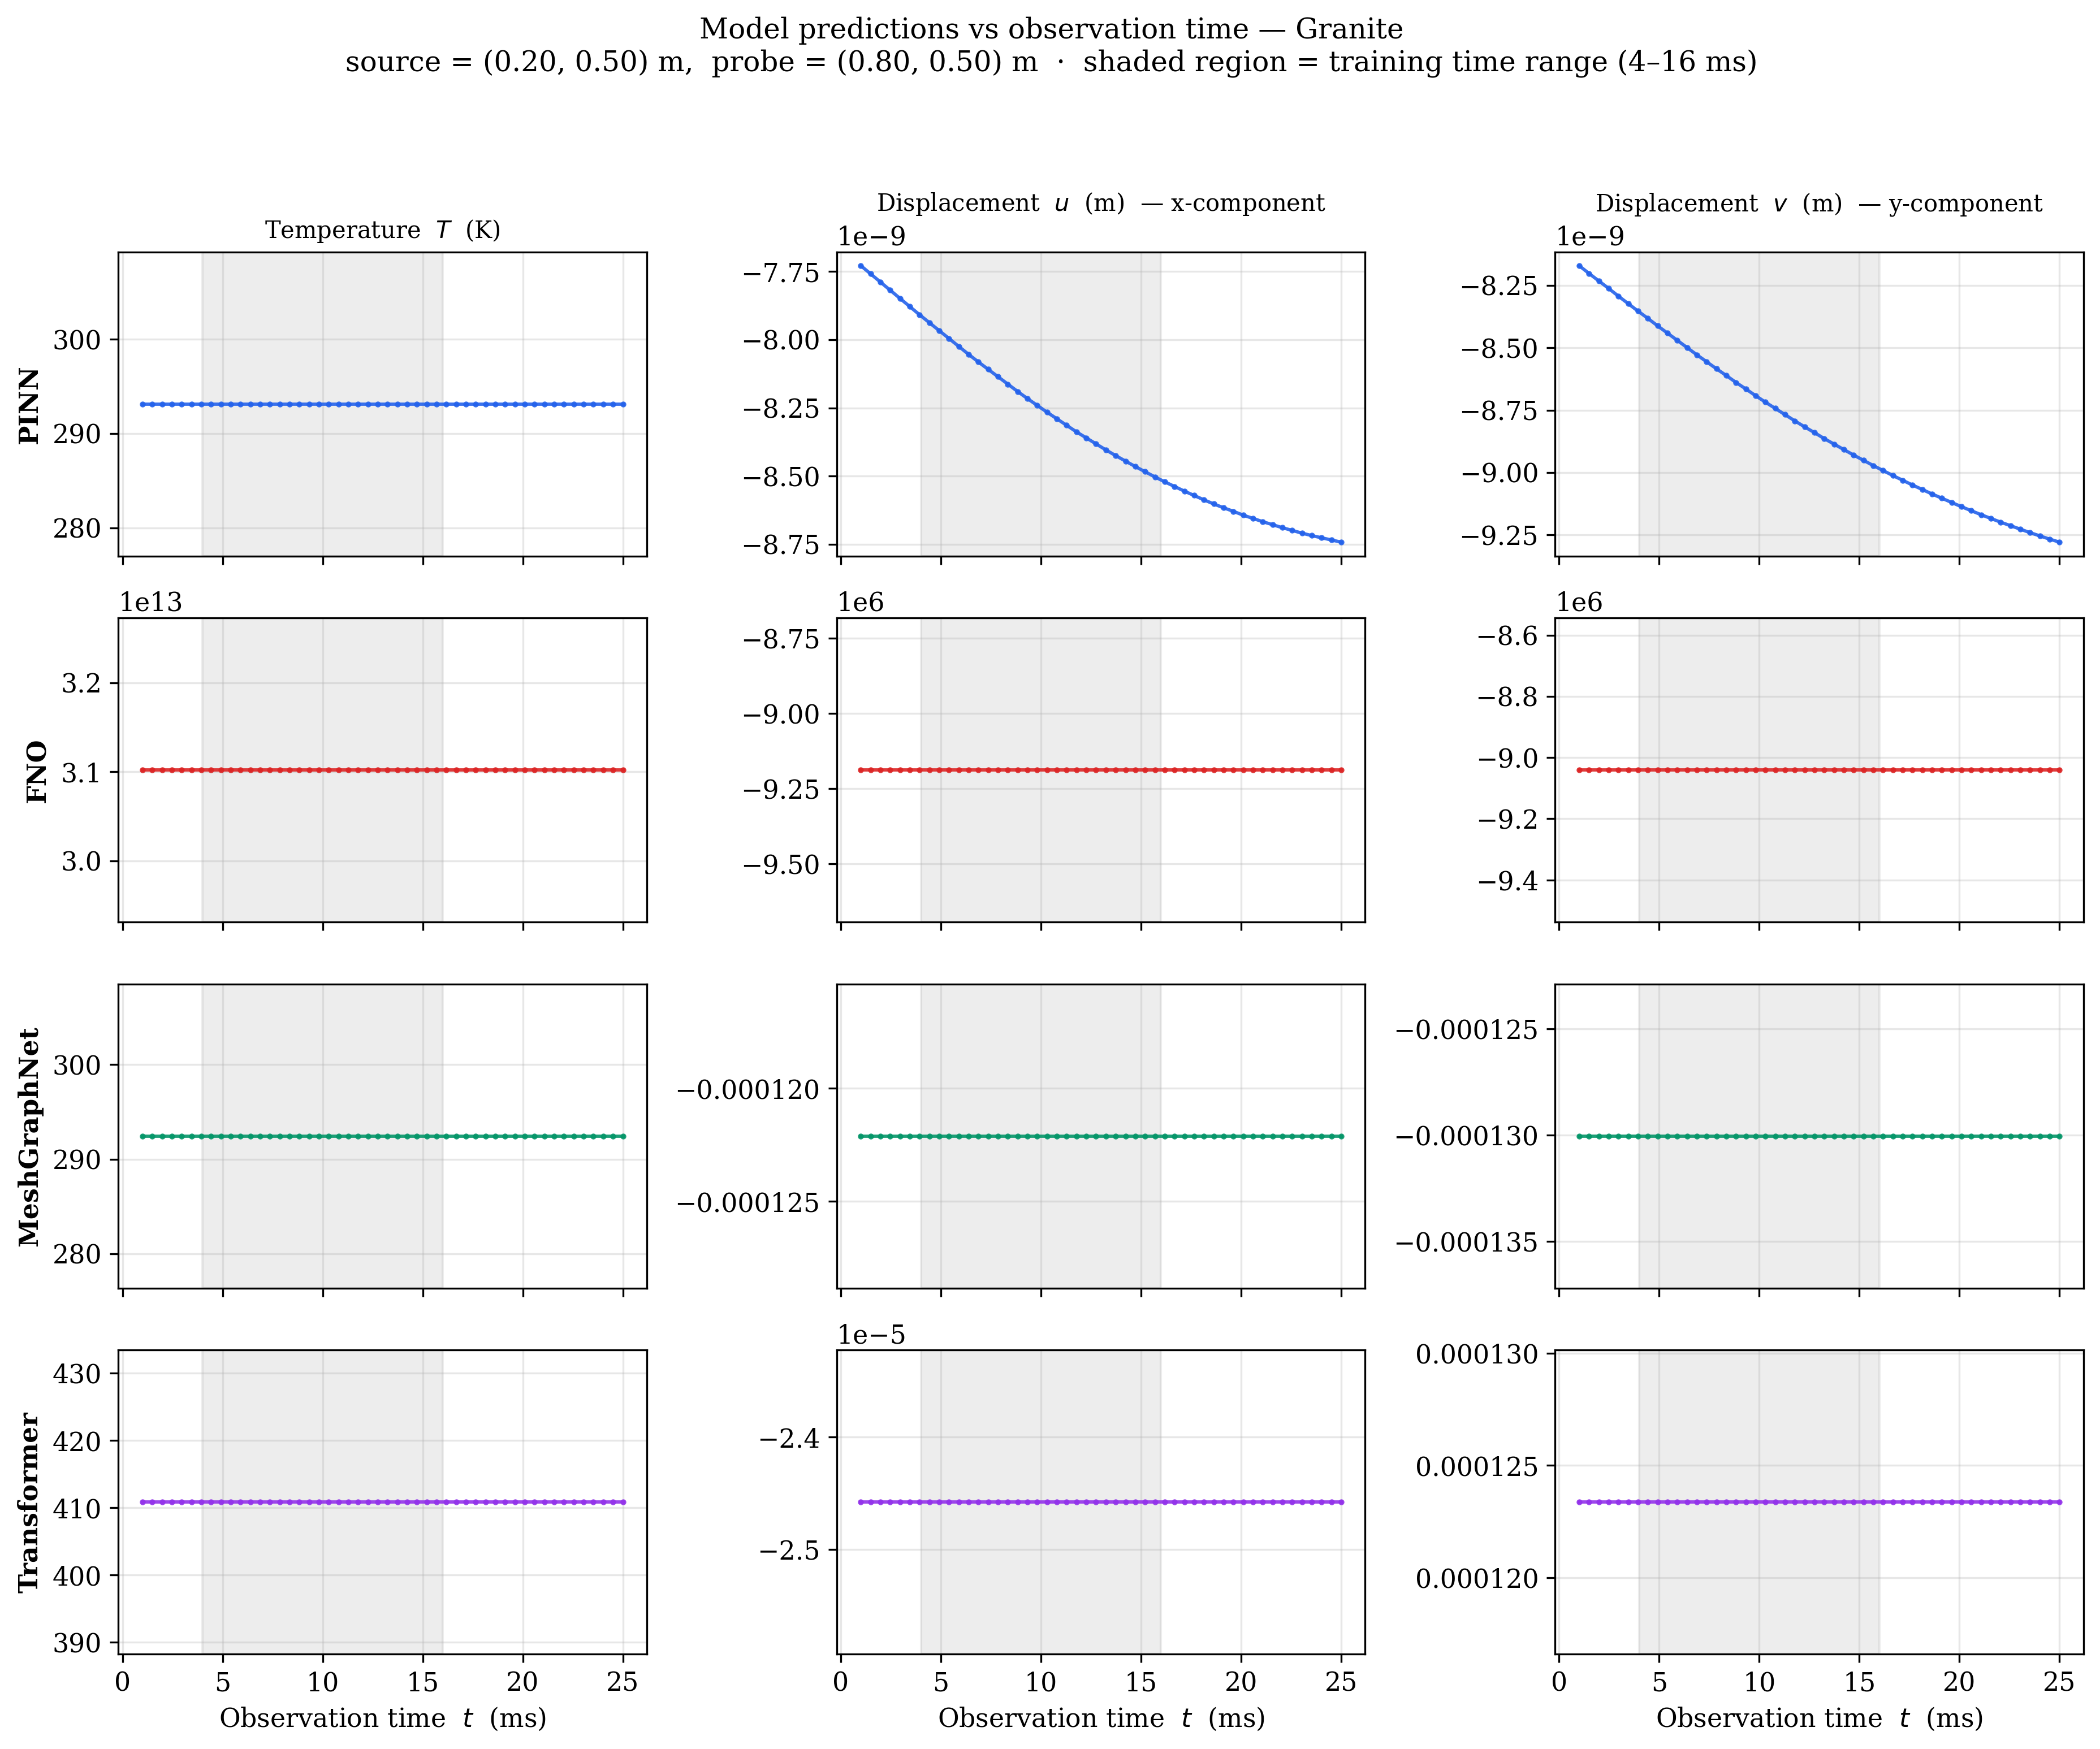
\includegraphics[width=\textwidth]{chapters/chapter6/figures/model_timeseries_granite.png}
\caption{Granite. PINN is the only route whose displacement traces
show a smooth time-dependent drift; the other three are flat across
the training time range.}
\label{fig:timeseries-granite}
\end{figure}

\begin{figure}[ht]
\centering
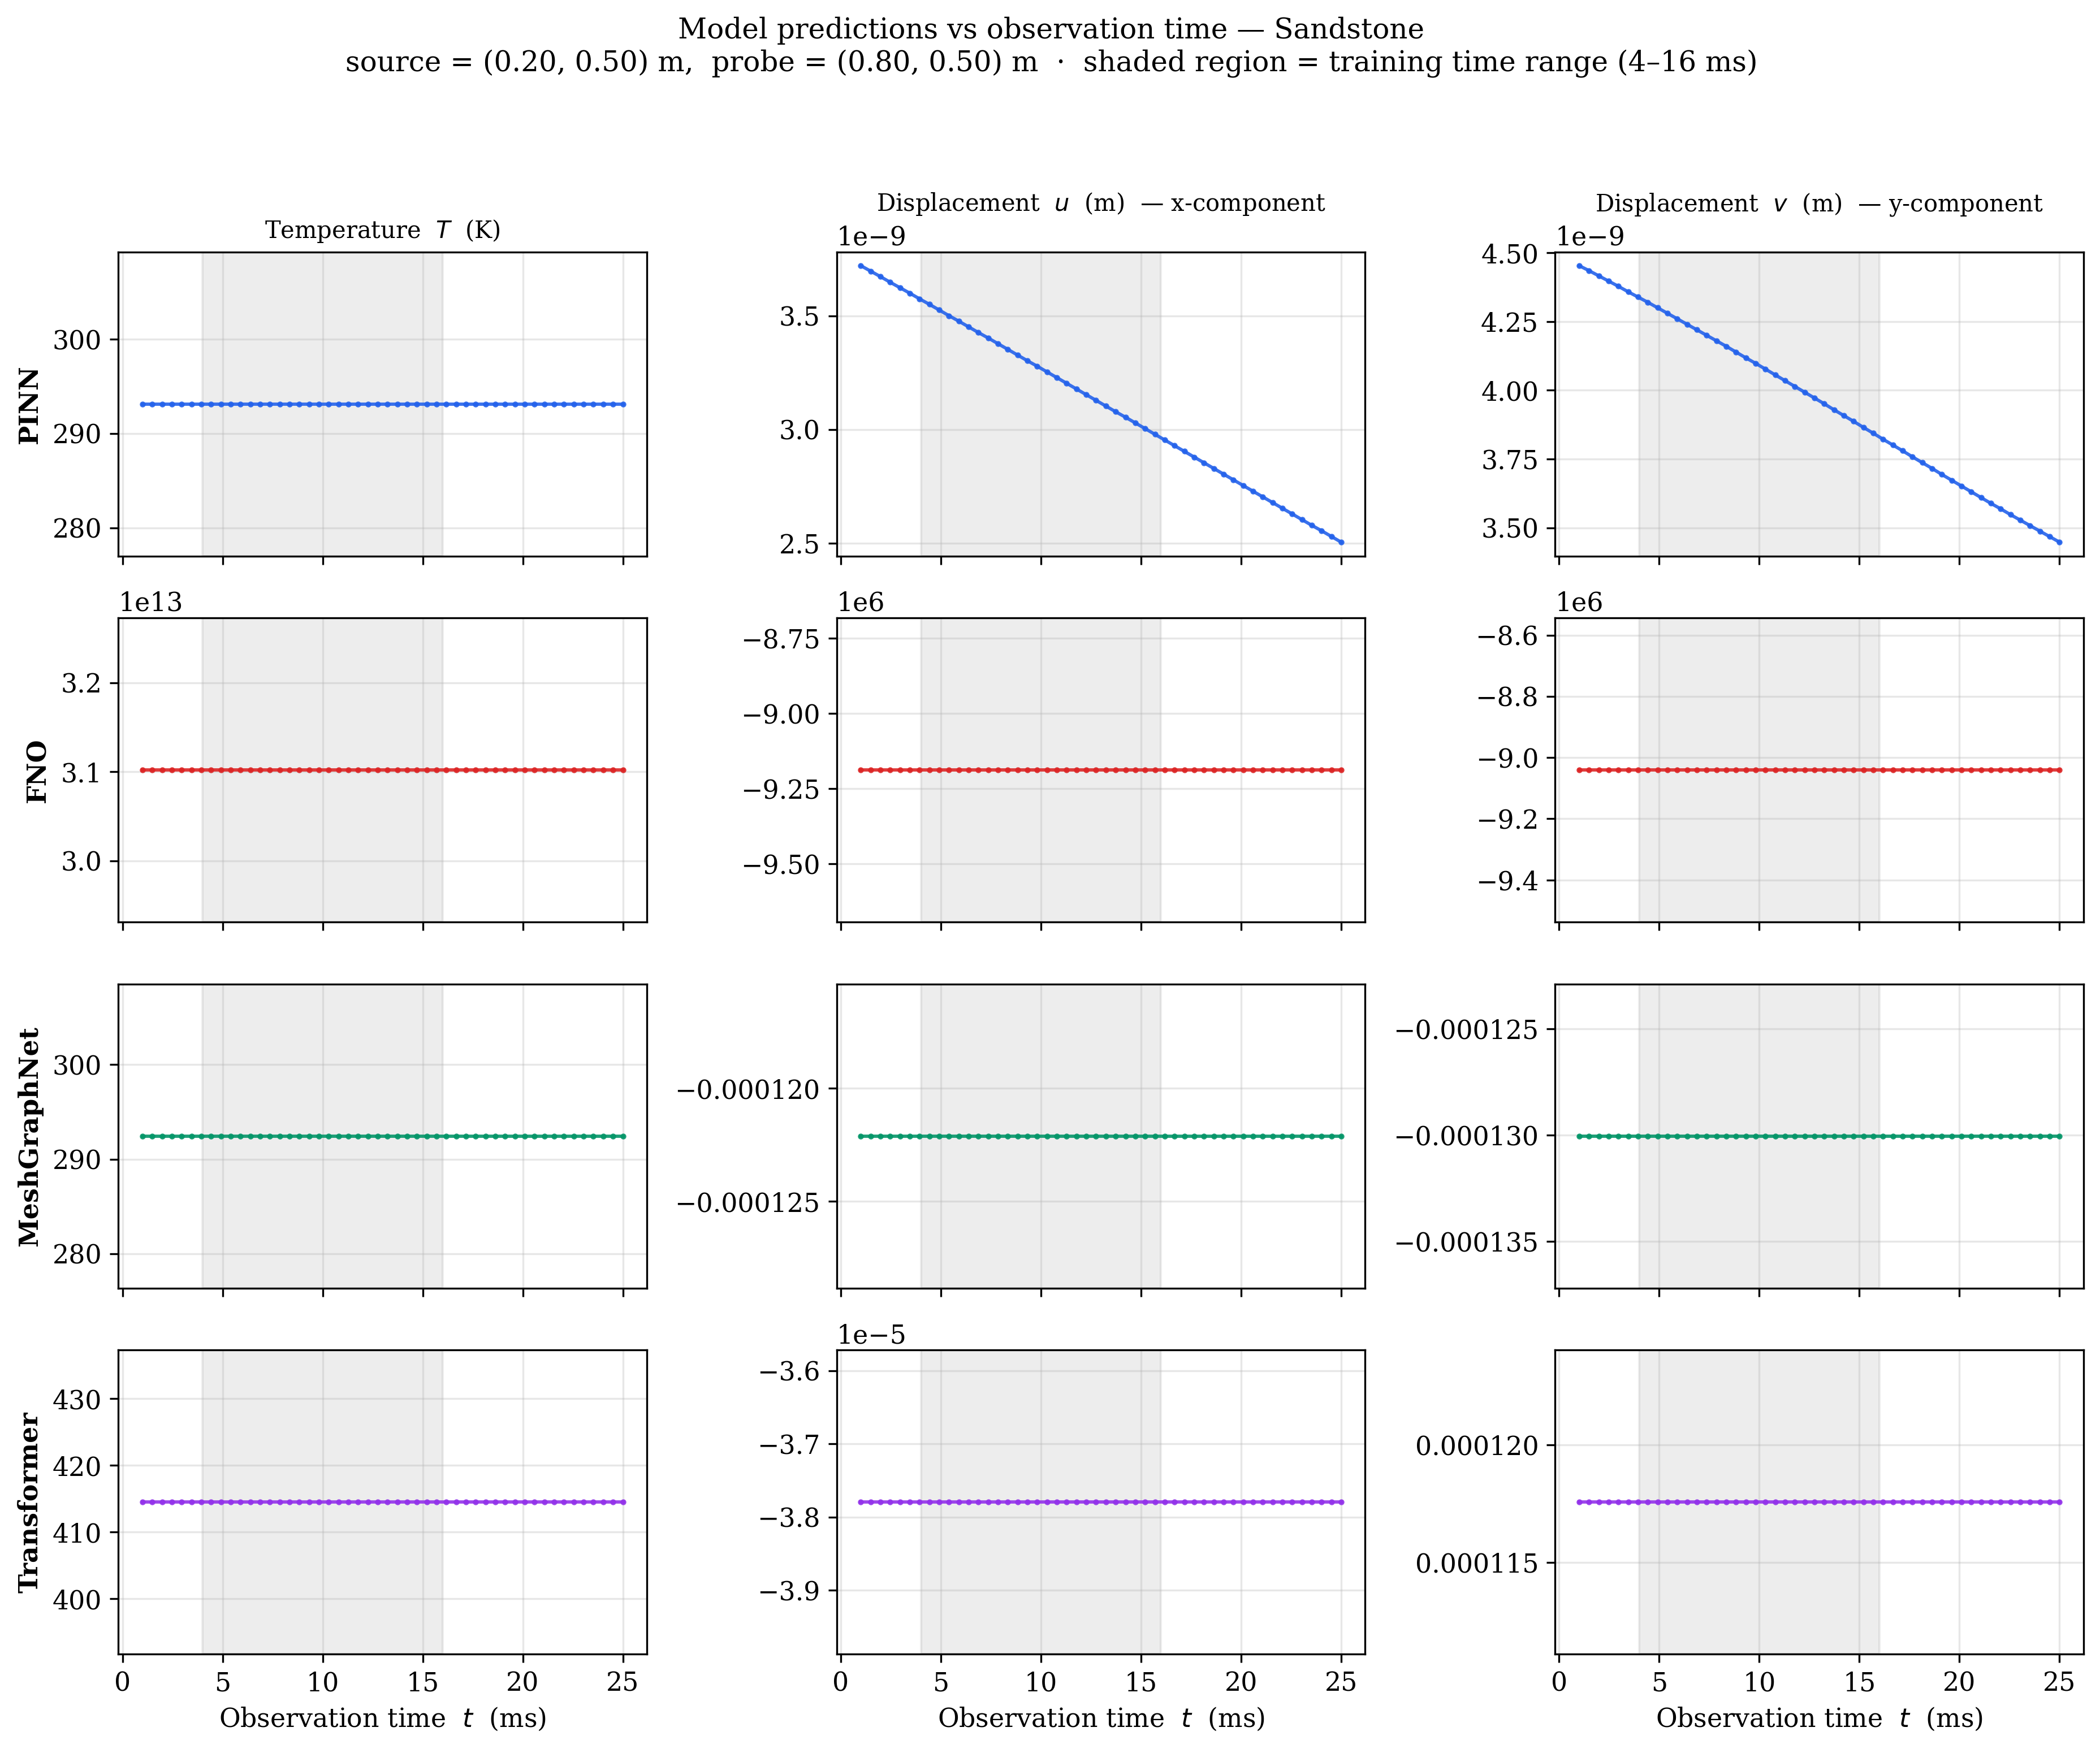
\includegraphics[width=\textwidth]{chapters/chapter6/figures/model_timeseries_sandstone.png}
\caption{Sandstone. Same layout as Figure~\ref{fig:timeseries-granite};
the qualitative pattern is identical across rocks.}
\label{fig:timeseries-sandstone}
\end{figure}

\begin{figure}[ht]
\centering
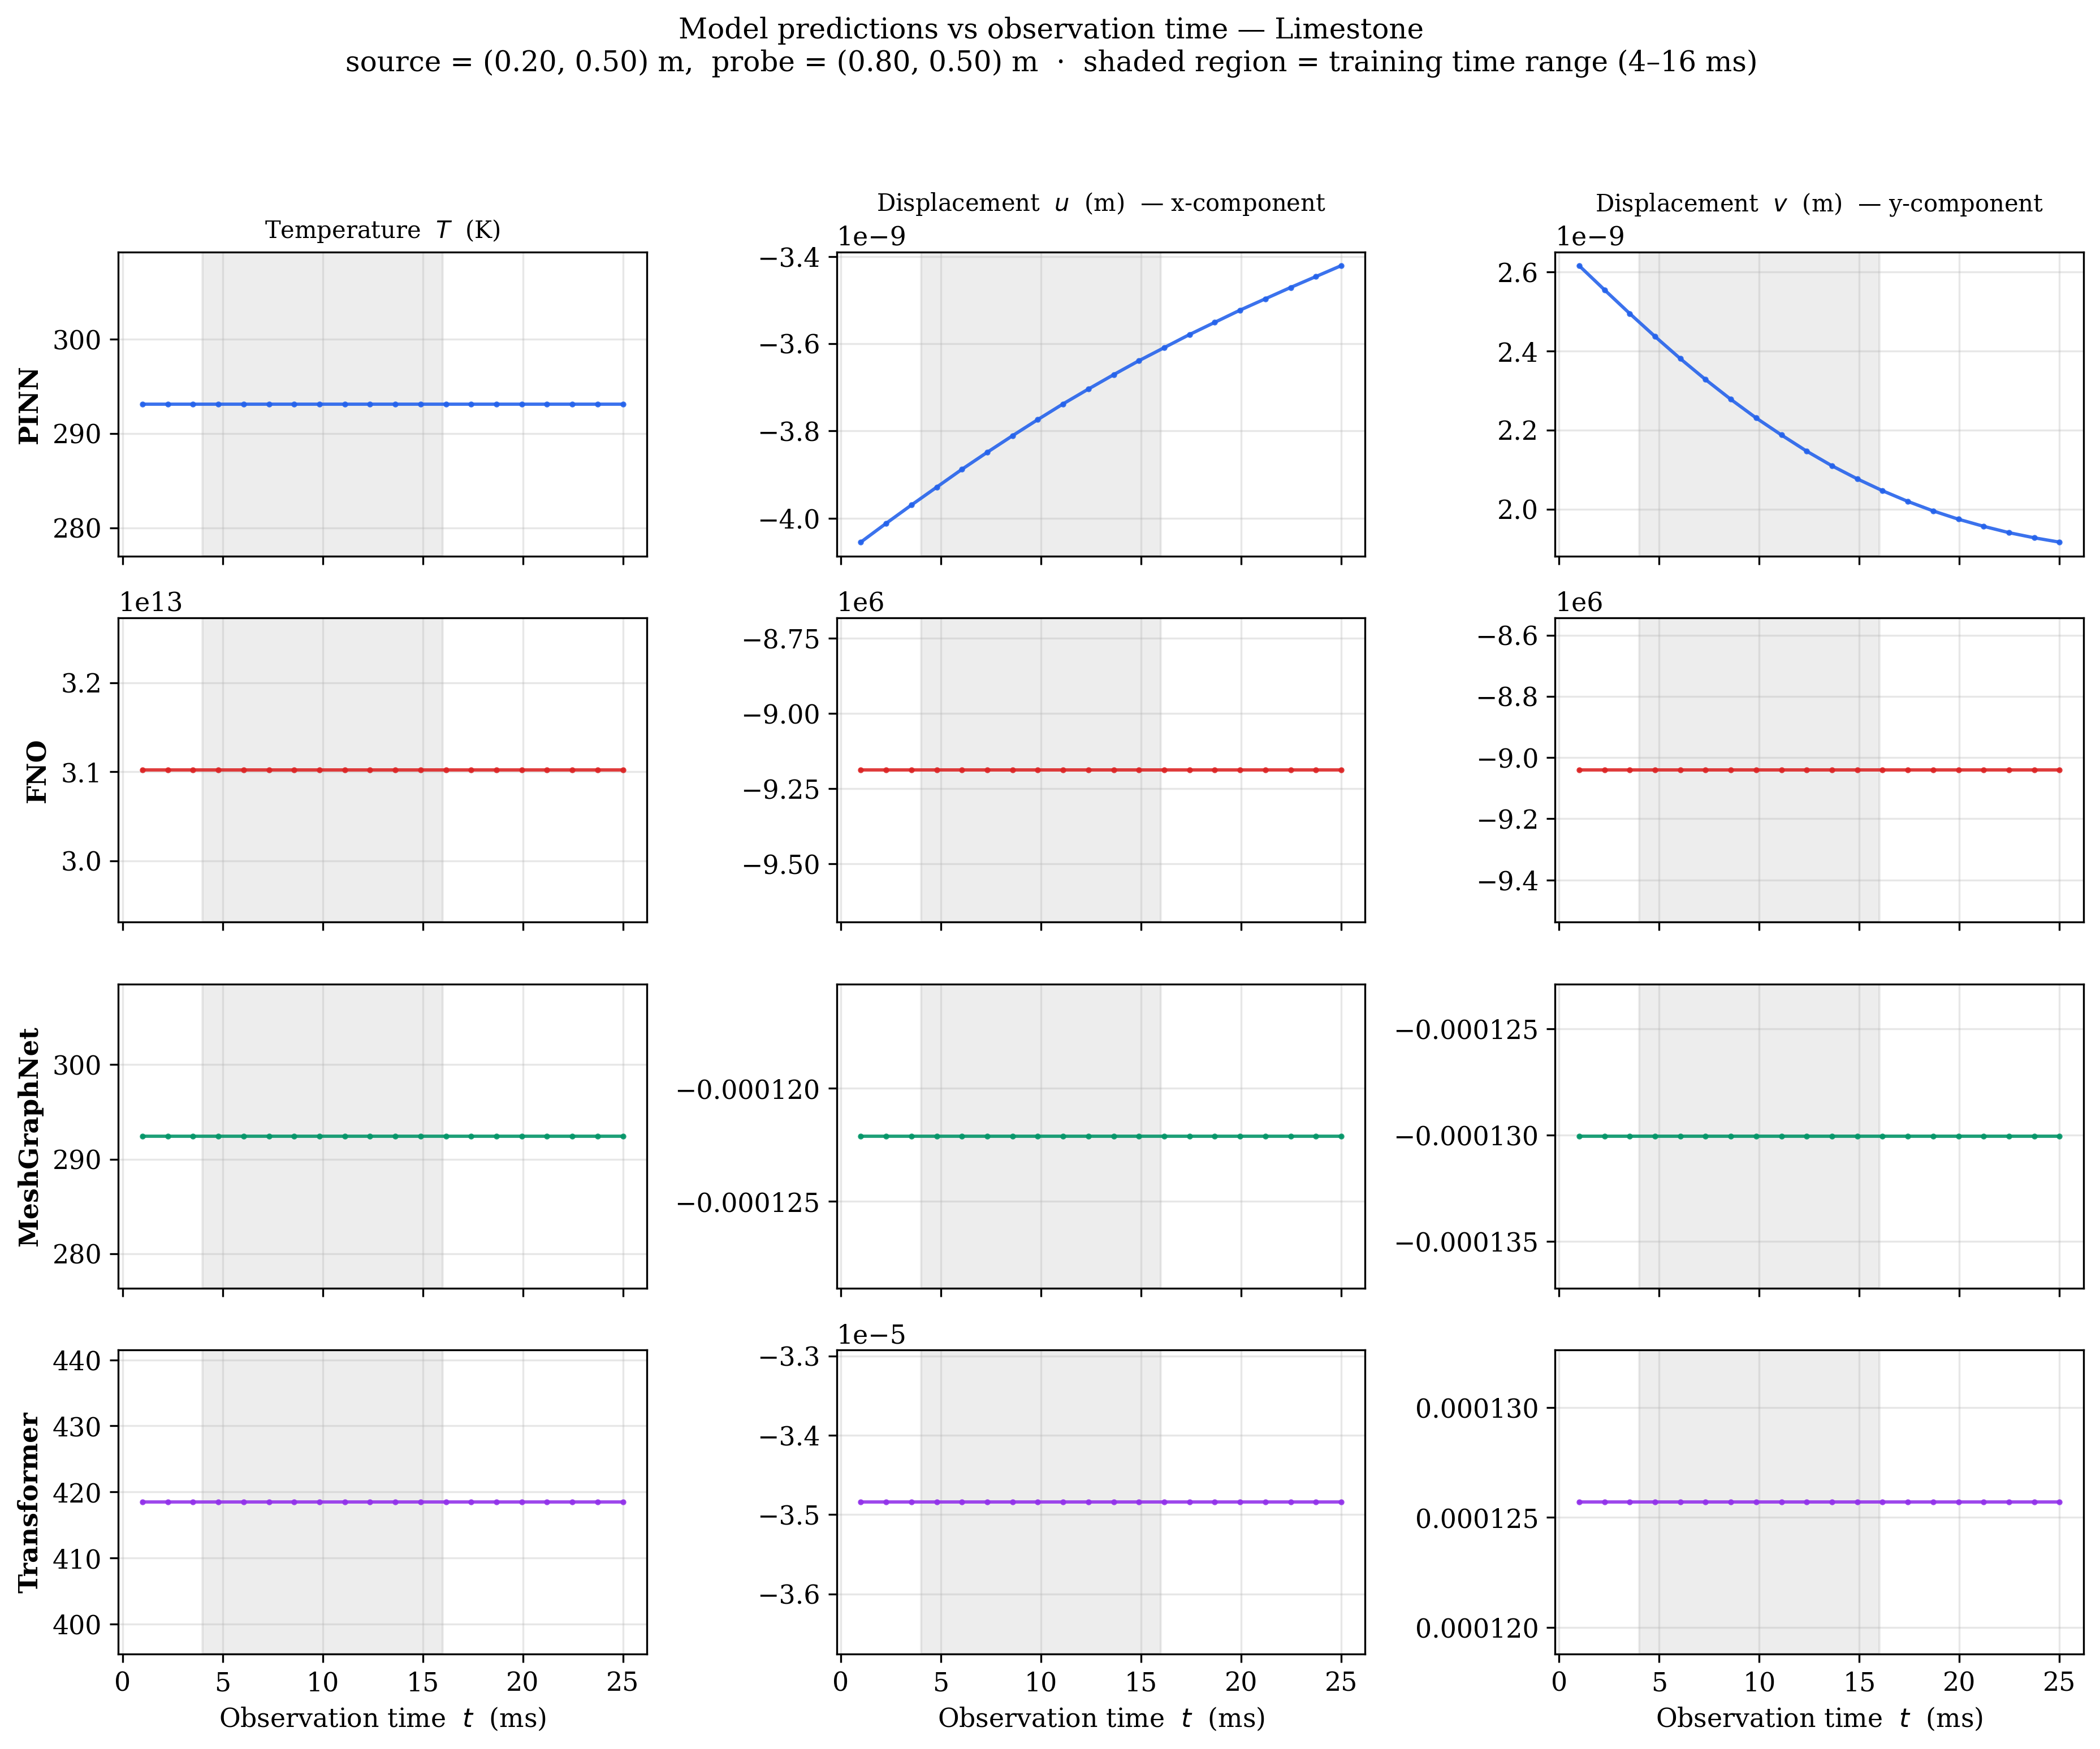
\includegraphics[width=\textwidth]{chapters/chapter6/figures/model_timeseries_limestone.png}
\caption{Limestone. Same layout as Figure~\ref{fig:timeseries-granite}.}
\label{fig:timeseries-limestone}
\end{figure}

The qualitative reading is the same for all three materials. Only
PINN reacts to the observation time at the probe: its displacement
$u$ and $v$ drift smoothly across the training time window because
its network takes $t$ as an explicit input feature and learns a
continuous function over it. The other three routes produce
essentially constant traces. The reasons differ:

\begin{itemize}
\item \textbf{FNO} maps the user's \texttt{observation.time\_s} to a
discrete \texttt{time\_index} in the dataset before assembling the
input field. Within the small time window that we sweep, the same
index is selected for every sample, so the predicted field at the
probe cell is byte-identical across the sweep. Increasing the time
window enough to cross a snapshot boundary would produce a step in
the trace, but not the smooth derivative information that the PINN
shows.

\item \textbf{MeshGraphNet} runs an autoregressive rollout of five
message-passing steps from the dataset's initial state. The rollout
horizon is hard-coded; the user's \texttt{observation.time\_s} does
not control how far the rollout runs. The route therefore returns the
same state at probe regardless of the requested time.

\item \textbf{Transformer} uses a fixed-length attention rollout that
also does not consume \texttt{observation.time\_s} as a per-call
duration. It is faster and more accurate than the deterministic
stubs, but it is still a fixed-horizon predictor.
\end{itemize}

This is not a plotting artefact: it is a real architectural property
of operator-learning surrogates for transient PDEs. Only the
point-wise PINN is natively continuous in time, because $t$ enters
the network in the same way $x$ and $y$ do. The other three are
operators between discrete time states. In the v2 contract every
route exposes the same scalar fields, so the comparison is fair, but
the comparison surfaces the difference clearly.

\subsection{Threats to validity and limitations}

The numerical values reported in this chapter should be read together
with the limitations of the experimental setup. First, the
ground-truth simulation is restricted to a single COMSOL pilot
(the heated rod in a rock domain of Chapter~4); the surrogates
therefore see only one geometric configuration during training, and
generalisation to genuinely different geological geometries is not
established by the present experiments. Second, the FNO route is
currently a 2D adaptation: every metric reported for FNO above is
affected by this restriction, and the route cannot be considered
2D-capable until its denormalisation and dimensionality issues are
resolved. Third, the inference latencies in Figure~\ref{fig:latency}
were measured on the host laptop in an interactive setting; on a
production GPU each route is expected to be at least an order of
magnitude faster, but the relative ordering of the four routes should
be preserved. Fourth, we do not attempt to compare the four
surrogates against an independent measurement of thermoelastic wave
propagation in a real geological formation; such a comparison would
require dedicated experimental work and lies outside the scope of
this thesis.

\subsection{Summary and recommendations}

Combining the metrics of the previous sections, three of the four
surrogates pass the basic sanity checks of the present evaluation.
The PINN baseline is the most conservative route and the cheapest to
evaluate, but it is also the route least sensitive to a change of
material. The Transformer-based neural operator is the route that
shows the strongest material-dependent response and the most consistent
two-dimensional directional output; at the price of being the
largest of the four models, it is also the most flexible in terms of
discretisation. MeshGraphNet sits between the two on most metrics and
offers a useful intermediate trade-off, with the caveat that its
autoregressive rollout is the most expensive at inference. The Fourier
neural operator, in its present implementation, cannot yet be ranked
on a comparable basis: it produces non-physical scales on the
displacement and temperature axes and a sign-inverted azimuth, and a
denormalisation correction is the first concrete implementation task
identified by this evaluation.

For the directional prediction problem of this thesis we therefore
recommend the PINN, MeshGraphNet and Transformer routes as the three
viable candidates for further investigation. PINN is the natural
physics-consistency baseline, MeshGraphNet is the natural choice for
irregular mesh-based simulations, and the Transformer-based operator
is the natural choice when the goal is to query the predictor at
arbitrary spatial coordinates that need not coincide with the COMSOL
mesh nodes. The Fourier neural operator should be revisited once an
FNO~2D variant with consistent output normalisation is implemented.
